\chapter{\huge{Drupal como consumidor de Servicios Web}}

Anteriormente hemos citado que nuestro sitio Drupal puede utilizar contenido externo a través de Servicios 
Web, utilizando los protocolos XML-RPC, REST, JSON, XML y RSS. Primero revisaremos con detalle un protocolo 
que puede ser usado por Drupal para comunicarse: el protocolo \textbf{SOAP (\textit{Simple Object Access Protocol})}.
Utilizaremos el módulo \textbf{Web Service Client}, ya que nos proporciona una interfaz para integrarnos 
con Servicios Externos. Se centra en la integración de operaciones de Servicios Web como acciones de reglas, 
pero también se puede utilizar como proveedor de datos para otros módulos. Debido a estas acciones, necesitaremos 
además el módulo \textbf{Rules}. La principal característica del módulo \textit{Web Service Client} es que 
viene con una interfaz de usuario que permite a los administradores del sitio crear descripciones de 
servicios REST y SOAP con sus respectivas operaciones y tipos de datos. Además, gracias a este módulo, 
podemos utilizar el \textbf{WSDL (\textit{Web Service Description Language})} del proveedor de Servicios Web.

WSDL es un lenguaje basado en XML que se utiliza para describir Servicios Web. Especifica dónde está el 
Servicio Web y el tipo de operaciones que éste implementa. Incluye especificaciones como el puerto 
o \textit{endpoint} dónde se encuentra el Servicio, el tipo de puerto o interfaz, operaciones permitidas y 
cómo es el mensaje permitido para cada operación. 

\section{SOAP en Drupal}

SOAP (Simple Object Access Protocol) es un protocolo orientado al acceso a objetos, que nos permite intercambiar 
información. Al igual que Al igual que XML-RPC y REST, el protocolo SOAP utiliza XML como formato de 
intercambio. Funciona básicamente como una base para nuestros interfaces de Servicios Web y permite construir 
un entorno de Servicio Web sobre el protocolo. Una de las principales ventajas de SOAP es que éste se encuentra 
de manera nativa a partir de la versión PHP5, con lo que no necesitaremos librarías externas.

SOAP funciona haciendo peticiones RPC (Remote Procedure Call) a un servidor externo. En esta sección veremos 
cómo integrar SOAP en Drupal para hacer peticiones a un WSDL de prueba, como el que provee la W3C para convertir 
métricas de temperatura.

La manera en la que la llamada se ejecuta es codificando el mensaje en formato XML por el cliente SOAP y 
ese mensaje es enviado a través del protocolo HTTP al servidor de aplicaciones Web externo. Para una mayor 
seguridad, se peude utilizar el protocolo HTTPS, por ejemplo, si estamos tratando con un Servicio Web de un banco.
   
Drupal se sirve de dos maneras diferentes a la hora de consumir utilizando SOAP. Drupal Soporta la extensión SOAP  
de PHP 5.x como mencionamos y de la extensión NuSOAP. NuSOAP no es una extensión SOAP sino más bien un conjunto 
de clases PHP que permiten la creación y consumo de Servicios Web. No se necesita instalar ninguna exptensión PHP 
para trabajar con NuSOAP y soporta las especificaciones de SOAP 1.1, pudiendo también generar documentos WSDL.


\subsection{Mensaje SOAP}

SOAP se basa en XML por lo que se considera de lectura humana, pero hay un esquema específico que debe 
ser respetado. Primero vamos a dividir un mensaje SOAP, eliminando datos para estudiar los elementos 
específicos que componen un mensaje SOAP.

\begin{verbatim}
<?xml version="1.0"?>
<soap:Envelope
 xmlns:soap="http://www.w3.org/2001/12/soap-envelope"
 soap:encodingStyle="http://www.w3.org/2001/12/soap-encoding">
 <soap:Header>
  ...
 </soap:Header>
 <soap:Body>
  ...
  <soap:Fault>
   ...
  </soap:Fault>
 </soap:Body>
</soap:Envelope>
\end{verbatim}

Esto podría parecer sólo un archivo XML normal, pero lo que lo convierte en un mensaje SOAP es el elemento 
raíz \textit{Envelope} con el espacio de nombres con http://www.w3.org/2001/12/soap-envelope. El atributo 
\textit{soap: encodingStyle} determina los tipos de datos utilizados en el archivo, pero SOAP en sí no 
tiene una codificación predeterminada.

\textit{soap:Envelope} es obligatorio, pero el elemento siguiente, \textit{soap: Header}, es opcional y 
por lo general contiene información relevante para la autenticación y gestión de sesiones. 
El protocolo SOAP no ofrece ninguna \textit{built-in} de autenticación, pero se lo permite a los desarrolladores 
incluirlo a través de esta etiqueta de cabecera.

A continuación está el elemento requerido \textit{soap:Body} que contiene el mensaje real RPC, incluyendo 
los nombres de método y, en el caso de una respuesta, los valores devueltos del método. El elemento 
\textit{soap:Fault} es opcional, si está presente, se tiene algún mensaje de error o información de estado 
para el mensaje SOAP y debe ser un elemento secundario de \textit{soap:Body}.

Ahora que ya entendemos los fundamentos de lo que constituye un mensaje SOAP, echemos un vistazo a la 
solicitud SOAP y los mensajes de respuesta. Vamos a comenzar con una petición.

\begin{verbatim}
<?xml version="1.0"?>
<soap:Envelope
 xmlns:soap="http://www.w3.org/2001/12/soap-envelope"
 soap:encodingStyle="http://www.w3.org/2001/12/soap-encoding">
 <soap:Body xmlns:m="http://www.yourwebroot.com/stock">
  <m:ObtenerPreciosMercado>
   <m:NombreMercado>IBM</m:NombreMercado>
  </m:ObtenerPreciosMercado>
 </soap:Body>
</soap:Envelope>
\end{verbatim}

El anterior es un ejemplo de mensaje SOAP de solicitud para obtener el precio de las acciones de una 
empresa en particular. Dentro de \textit{soap:Body} se observa el elemento \textit{ObtenerPreciosMercado} que es 
específico de la aplicación. No es un elemento SOAP, y toma su nombre de la función en el servidor que se 
llamará para esta solicitud. \textit{NombreMercado} también es específico de la aplicación y es un argumento 
para la función.

El mensaje de respuesta es similar a la solicitud:

\begin{verbatim}
<?xml version="1.0"?>
<soap:Envelope
 xmlns:soap="http://www.w3.org/2001/12/soap-envelope"
 soap:encodingStyle="http://www.w3.org/2001/12/soap-encoding">
 <soap:Body xmlns:m="http://www.yourwebroot.com/stock">
  <m:ObtenerPreciosMercadoResponse>
   <m:Precio>183.08</m:Precio>
  </m:ObtenerPreciosMercadoResponse>
 </soap:Body>
</soap:Envelope>
\end{verbatim}

En el elemento \textit{soap:Body} hay un elemento \textit{ObtenerPreciosMercadoResponse} con un hijo \textit{Precio}, 
que contiene los datos de retorno. Como es de suponer, tanto \textit{ObtenerPreciosMercadoResponse} tanto \textit{Precio} 
son específicos para esta aplicación.
 
Ahora que ya hemos visto un ejemplo de petición y respuesta y entendemos la estructura de un mensaje SOAP, 
vamos a instalar NuSOAP y construir un cliente SOAP y el servidor para probar la generación de este tipo de 
mensajes.

\subsection{Instalando SOAP en PHP}

Antes de utilizar SOAP en frameworks de PHP, como Drupal, hay que asegurarse de que la extensión SOAP 
está instalado y habilitada en nuestro servidor. SOAP se ejecuta como una extensión de PHP. Podemos revisar 
el archivo de configuración PHP, o pulse en el link para comprobar su versión de PHP, en su la página de 
informes de Drupal para comprobar la configuración de PHP y ver si SOAP es habilitado. 

En muchos servidores compartidos o dedicados, la extensión debe ser auto-activada, por lo que no tendrás que 
hacer nada especial para que funcione. Sin embargo, en caso de que la extensión no está activada, tendremos que habilitarla.
Podemos abrir el fichero de configuración de PHP (\textit{php.ini}) y buscar el siguiente texto desde en el apartado 
\textit{Configure Command}: \verbatim{--enable-soap}. Este comando le muestra si SOAP está habilitado. 

A continuación, podemos acceder a la página de información de PHP (utilizando el método \textit{phpinfo()}) y 
buscar la sección específica para la extensión SOAP y deberíamos tener algo como lo siguiente:

\begin{figure}
  \centering
    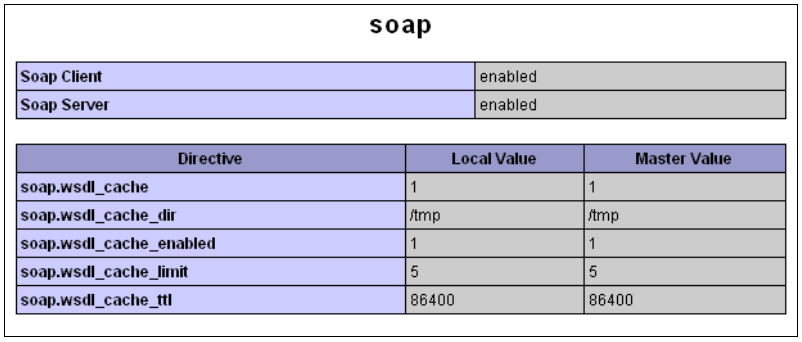
\includegraphics[scale=0.2]{Assets/Soap/Imagenes/phpinfo.png}
  \caption{Extensión SOAP}
\end{figure}
